\documentclass{dhbenelux}

\usepackage{booktabs} % for toprule, midrule, bottomrule in tables
\usepackage{authblk} % for multiple authors and affiliations
\usepackage{graphicx} % to include graphics with \includegraphics
\usepackage{courier}
\usepackage{array}
\usepackage{listings}
\usepackage{tabularx}
\usepackage{longtable} % For long tables (if needed)
\usepackage{adjustbox}
\usepackage{amsmath} % for math equations
\usepackage{algorithm}
\usepackage{algpseudocode}
\usepackage{verbatim}
\usepackage{mathtools} % additional math features
%% \usepackage{cleveref} % smart cross-referencing
\usepackage{hyperref} % put hyperref last

\author[1]{Anirudh Dambal}
\author[1]{Harish Patil}
\author[1]{Pavan Bhakta}
\author[1]{Anusha Adarakatti}

\affil{School of Computer Science and Engineering,
KLE Technological University, Hubballi, Karnataka, India, 580031}

\title{Code to Code Conversion from Java to Python
Using T5-Small}

\begin{document}

\maketitle

\section{Introduction}

Code-to-code translation addresses real-world challenges such as adapting legacy systems to new technologies, improving code maintainability, and increasing cross-language collaboration. For example, businesses transitioning from Java to Python may aim to leverage Python’s rich data science libraries without discarding years of development in Java. This requires reliable methods to convert existing codebases accurately while preserving their original logic and functionality.

Domain-Specific Languages (DSLs) like Spark, NumPy, TACO, and P4 have changed the face of modern software development process by providing optimizations and abstractions tailored to specific applications. They improve code clarity, usability, and performance. However, they often require rewriting legacy code—a very tedious and error-prone process that risks changing the original behavior. Transpilation, or translating code between high-level languages, remains a significant challenge.

Recent advancements in Large Language Models (LLMs), such as BERT, GPT-3, and T5, have been promising in the automation of programming tasks like code generation and repair. Still, reliable code translation remains a challenge because most models lack robustness and correctness guarantees. In addition, formal verification tools depend on niche languages like SMT-LIB and Dafny, which are underrepresented in LLM training datasets, thus limiting their practical application.

The core challenge lies in translating code between high-level languages with distinct syntax and semantics, such as Java and Python. Current transpilation methods demand manual effort and expertise, which reduces efficiency and increases the risk of errors. While LLMs offer potential solutions, existing models often fail to address these limitations in real-world scenarios.

The main goals of this paper are to curate a dataset of paired Java and Python programs for training. The study attempts to determine the efficacy of the T5 model in automating the translation of Java to Python code and addresses the practical challenges encountered by developers, such as syntactic and semantic differences between the two languages.

The rest of the paper is organized as follows: Section 2 reviews related work, focusing on advancements in machine learning techniques for programming tasks. Section 3 outlines the proposed methodology, including dataset preparation and model training. Section 4 presents experimental results, analyzing the T5 model's performance in code translation. Section 5 discusses key findings and future research directions. Finally, Section 6 concludes with insights into the study's contributions.

\section{Related Work}

The application of machine learning models to programming tasks has seen significant advancements in recent years. Early research focused on representing code for machine learning purposes, leveraging hierarchical structures such as Abstract Syntax Trees (ASTs). Researchers like Tai et al. (2015) introduced Tree-LSTM models, which encode tree structures by processing nodes iteratively. Tree-LSTM extends the standard LSTM to handle tree-structured data by defining cell states and hidden states for each node \( i \) based on its child nodes \( C(i) \). The formula for this is expressed in equation~\ref{eq:tree-lstm}:
\begin{equation}
h_i, c_i = \text{TreeLSTM}(x_i, \{h_{j}, c_{j} \,|\, j \in C(i)\}).
\label{eq:tree-lstm}
\end{equation}

This innovation laid the groundwork for program analysis and transformation. A schematic representation of the Tree-LSTM architecture can be illustrated in Figure~\ref{fig:tree-lstm}.

\begin{figure}[h]
    \centering
    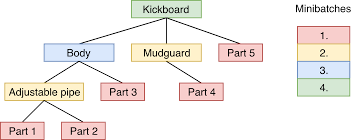
\includegraphics[width=0.8\textwidth]{Images/1.png} % Replace with actual Tree-LSTM flowchart
    \caption{Tree-LSTM Architecture for AST Processing}
    \label{fig:tree-lstm}
\end{figure}

Chen et al. (2018) extended this approach by proposing a tree-to-tree encoder-decoder framework tailored specifically for code. This framework enabled structured transformations between different tree representations, such as converting an AST of one language into another. The encoder mapped the source tree \( T_s \) into a latent representation \( z \), and the decoder reconstructed the target tree \( T_t \). This process is expressed in equation~\ref{eq:tree-to-tree}:
\begin{equation}
z = f_{\text{encoder}}(T_s), \quad T_t = f_{\text{decoder}}(z).
\label{eq:tree-to-tree}
\end{equation}

Drissi et al. (2018) refined these ideas further by introducing the Left-Child Right-Sibling (LCRS) representation, simplifying tree encoding by reducing tree structures into binary trees, which proved effective for program translation tasks.

\begin{figure}[h]
    \centering
    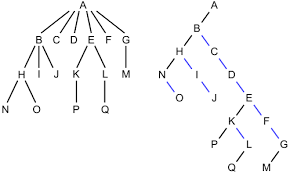
\includegraphics[width=0.8\textwidth]{Images/2.png} % Replace with actual flowchart for tree-to-tree model
    \caption{Tree-to-Tree Encoder-Decoder Framework for Code Transformation}
    \label{fig:tree-encoder-decoder}
\end{figure}

The advent of neural machine translation (NMT) frameworks inspired new applications beyond natural language. Tufano et al. (2018) explored automated bug fixing by applying NMT to software maintenance tasks. They mined GitHub for bug-fix commits and abstracted code changes into generalizable patterns. Using tools like GumTree for edit tracking, they trained models capable of generating patches resembling developer edits. The loss function used to train the model, minimizing syntactic and semantic differences between generated and ground truth patches, is expressed in equation~\ref{eq:nmt-bug-fixing}:
\begin{equation}
\mathcal{L} = \sum_{i=1}^N \text{CrossEntropy}(\hat{y}_i, y_i),
\label{eq:nmt-bug-fixing}
\end{equation}
where \( \hat{y}_i \) is the predicted token and \( y_i \) is the actual token. Their approach achieved high syntactic correctness and underscored the utility of NMT in learning transformations at the AST level.
\begin{figure}[h]
    \centering
    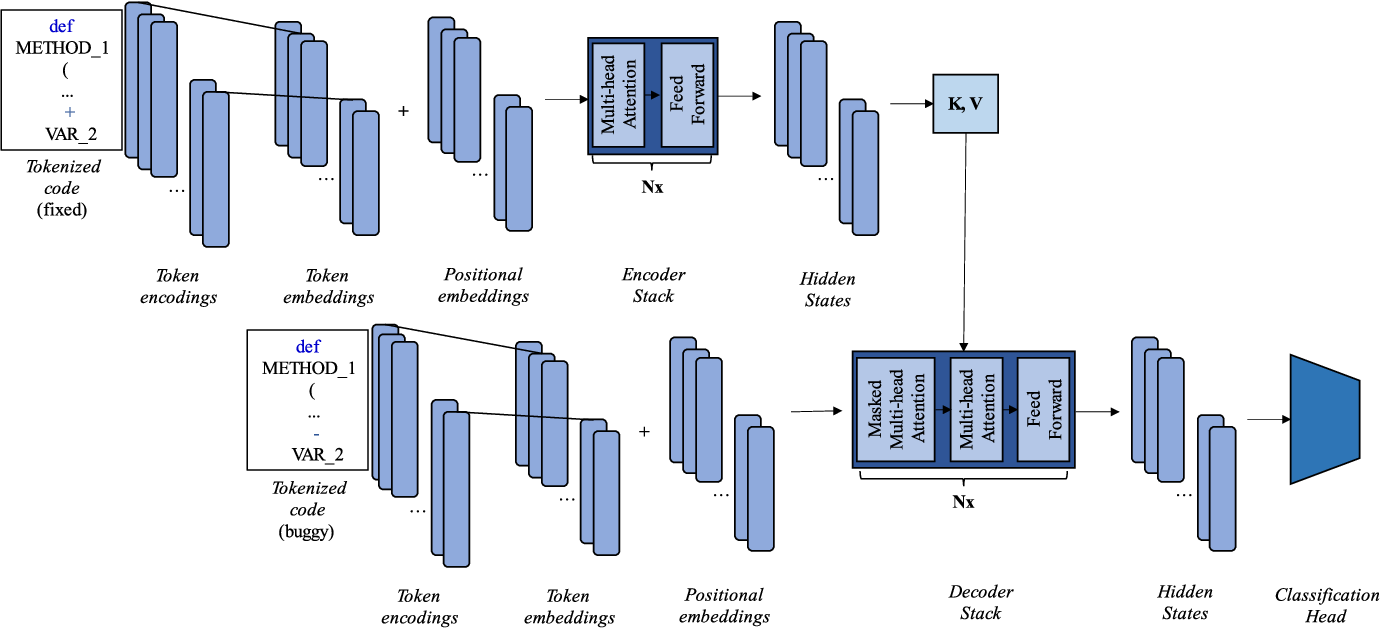
\includegraphics[width=0.8\textwidth]{Images/3.png} % Replace with NMT bug fixing diagram
    \caption{Neural Machine Translation for Automated Bug Fixing}
    \label{fig:nmt-bug-fixing}
\end{figure}

Lachaux et al. (2020) introduced TransCoder, a system for translating functions between programming languages without requiring parallel training data. By leveraging monolingual source code and unsupervised learning techniques, TransCoder captured language-specific patterns. The objective was to minimize a combined reconstruction and translation loss, as described in equation \ref{eq:loss}:
\begin{equation}
\mathcal{L} = \mathcal{L}_{\text{reconstruction}} + \mathcal{L}_{\text{translation}},
\label{eq:loss}
\end{equation}
where \( \mathcal{L}_{\text{reconstruction}} \) ensures that monolingual data reconstructs correctly, and \( \mathcal{L}_{\text{translation}} \) aligns the latent spaces of source and target languages. TransCoder outperformed rule-based systems, showcasing robust language-agnostic representations.

\begin{figure}[h]
    \centering
    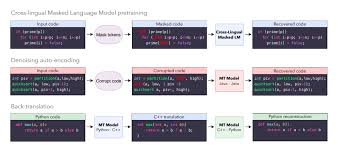
\includegraphics[width=0.8\textwidth]{Images/4.jpg}
    \caption{TransCoder Framework for Unsupervised Code Translation}
    \label{fig:transcoder}
\end{figure}

Katz et al. (2019) addressed decompilation, converting low-level code to high-level programming languages. Traditional decompilers relied on expert-crafted rules, but Katz et al. proposed a neural model to reverse compiler processes. Their NMT-based framework achieved high success rates in translating LLVM IR and x86 assembly back to source code, with substantial improvements over rule-based systems. 

More recently, Armengol-Estapé et al. (2021) explored transformer models for compilation tasks, marking a shift towards leveraging large pre-trained models. Transformers, with their self-attention mechanisms, allowed efficient modeling of long-range dependencies in code. The attention mechanism is expressed in equation \ref{eq:attention}, as shown below:
\begin{equation}
\text{Attention}(Q, K, V) = \text{softmax}\left(\frac{QK^\top}{\sqrt{d_k}}\right)V,
\label{eq:attention}
\end{equation}
where \( Q \), \( K \), and \( V \) are query, key, and value matrices, and \( d_k \) is the dimensionality of the keys. These models opened new possibilities for tasks like code generation, translation, and repair.

\begin{figure}[h]
    \centering
    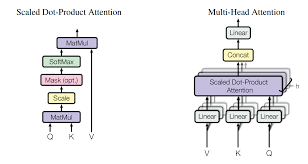
\includegraphics[width=0.8\textwidth]{Images/5.png} % Replace with transformer-based model diagram
    \caption{Transformer Model for Compilation Tasks}
    \label{fig:transformer-code}
\end{figure}

These advancements collectively illustrate the evolution of machine learning techniques for programming tasks. From tree-based models to NMT and transformers, each step has contributed to a deeper understanding of how programs can be represented, translated, and optimized, forming the foundation for the methods explored in this work.


\section{Proposed Work}

This work presents a transpilation framework for automatic translation between high-level programming languages, namely Java and Python, using a fine-tuned T5-small model. The framework employs the encoder-decoder architecture of T5-small to capture syntactic and semantic differences between these languages. The implementation focuses on training and inference, achieving a robust pipeline for translating Java code into Python.

\subsection{Dataset preparation}
The data preparation methodology involves a series of systematic steps designed to generate and balance pseudocode, Python, and Java code from text descriptions using Gemini Generative AI. The AI is guided to produce language-agnostic code that avoids language-specific built-in functions and dependencies, thus enhancing cross-language versatility. Data management is done using the pandas library, where generated outputs are appended to maintain an equal representation across different programming languages. The process has mitigated rate limit issues due to APIs; \texttt{time.sleep} is integrated for a delay between API calls to ensure smooth-running operations, and dynamic adjustment is carried out in regard to changing dataset sizes for this process. Finally, validation and saving of the last dataset are completed as a dependable source for future cross-language training and subsequent computational analysis.

\begin{figure}[h!]
\centering
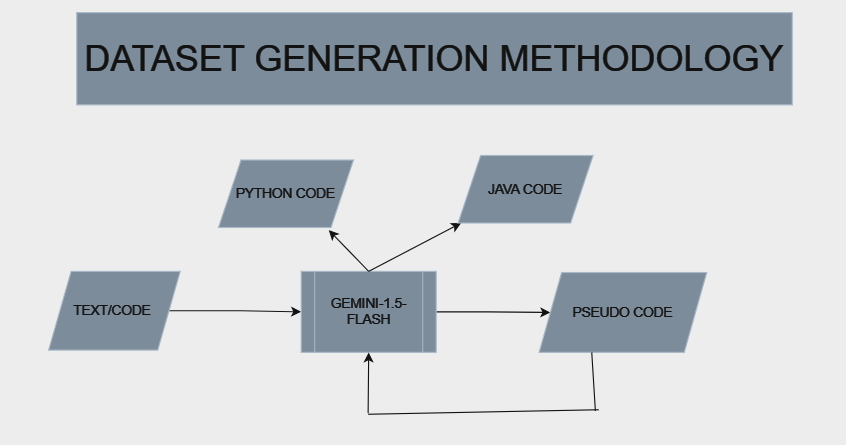
\includegraphics[width=0.7\textwidth]{dataset_methodology.png} % Replace with actual flowchart file
\caption{Dataset Preparation Methodology}
\label{fig:dataset-methodology}
\end{figure}

\subsubsection{Algorithms}

The process of data preparation is done through several key steps to ensure the quality of the generated data as being both balanced and effective. We \textbf{integrate the Gemini API}, which creates structured API calls that transform pseudocode into corresponding code snippets, starting with Java and Python code generation from pseudocode instructions. Next, we \textbf{balance the data} so that we have equal numbers of pairs of Java and Python code by keeping the dataset fair to allow for cross-language training. Last but not least, we implement a 4-second delay between requests in order not to hit \textbf{API rate limits}. That's essential to avoid hitting any breaks during the process. These steps combined result in a dataset that is reliable, well-rounded, and ready for further use.

\begin{algorithm}
\caption{Generate Balanced Code Pairs from Text Input}
\label{alg:balanced_code_pairs}
\begin{algorithmic}[1]
\Require Two CSV files: \texttt{xlcost\_text\_to\_code.csv}, \texttt{Dataset.csv}
\Ensure \texttt{Dataset.csv} updated with balanced and effective code pairs

\State Load data from \texttt{xlcost\_text\_to\_code.csv} and \texttt{Dataset.csv}
\State Configure API key and initialize the Generative AI model
\State Determine the total number of rows in the dataset, $n$
\For{each text sample in \texttt{data["text"][1:n]}}
    \State \textbf{Generate pseudocode} using the text input
    \State Wait for 5 seconds
    \State \textbf{Generate Python code} from the pseudocode
    \State Wait for 5 seconds
    \State \textbf{Generate Java code} from the pseudocode
    \State Wait for 5 seconds
    \State Structure the generated data into a new DataFrame
    \State Append the new DataFrame to the existing dataset
    \State Save the updated dataset to \texttt{Dataset.csv}
\EndFor
\State \textbf{Output:} Updated \texttt{Dataset.csv}
\end{algorithmic}F
\label{alg:generate-balanced-code}
\end{algorithm}

Generative AI, for example, Google Gemini-1.5, makes use of advanced large-scale language models trained on multiple datasets to process natural language prompts and generate programmatic code in multiple languages. The technology allows for context-aware mechanisms to be used for accurate and versatile code generation. For data handling, the system uses Pandas, a Python-based data manipulation library to efficiently read, update, and save datasets in structured formats like.csv. It offers concatenation and indexing functionalities that can append newly created outputs including pseudo-code, Python and Java code into the system iteratively. This approach to workflow automation allows more scalability and consistency across different prompts. Moreover, for cross-language compatibility, this model designs its prompts such that they do not rely on the built-in functions that exist in other languages, allowing easy translations across languages.

The self-attention mechanism is a fundamental component of the transformer architecture, computing relative relationships between input tokens according to the following equation, as shown in equation \ref{eq:self-attention}:

\begin{equation}
\text{Self-Attention}(Q, K, V) = \text{softmax}\left(\frac{QK^\top}{\sqrt{d}}\right)V.
\label{eq:self-attention}
\end{equation}

where \( Q \) (query), \( K \) (key), and \( V \) (value) matrices are derived from input embeddings through learned transformations. The scaling factor \( \sqrt{d} \) stabilizes softmax probabilities, focusing computational resources on the most relevant tokens. Layer normalization further stabilizes model training by normalizing input vectors through the formula, as expressed in equation \ref{eq:layer-norm}:

\begin{equation}
\text{Norm}(x) = \frac{x - \mu}{\sigma + \epsilon}.
\label{eq:layer-norm}
\end{equation}

where \( \mu \) is the mean, \( \sigma \) is the standard deviation, and \( \epsilon \) is a small constant for numerical stability. The feedforward layers in transformers enhance the model’s non-linear learning capacity, expressed as shown in equation \ref{eq:ffn}:

\begin{equation}
\text{FFN}(x) = \text{max}(0, xW_1 + b_1)W_2 + b_2.
\label{eq:ffn}
\end{equation}

where \( W_1 \), \( W_2 \) are weight matrices, and \( b_1 \), \( b_2 \) are bias vectors. Lastly, cross-entropy loss optimizes the model by minimizing the error between true labels (\( y_i \)) and predictions (\( \hat{y}_i \)) using the formula in equation \ref{eq:cross-entropy}:

\begin{equation}
L = -\sum_{i=1}^N y_i \log(\hat{y}_i).
\label{eq:cross-entropy}
\end{equation}

These interconnected methodologies ensure the system’s robustness and precision in generating cross-compatible, efficient programmatic solutions.


The process begins with feeding a set of text instructions into the Gemini model to generate pseudocode, an abstract, language-agnostic representation of the program's logic. The pseudocode is then fed again into Gemini to produce executable code snippets in both Java and Python. This ensures that the generated code snippets remain independent of specific language attributes or properties, such as Python's \texttt{.reverse()} method. This is done to make the output more versatile and compliant with wider standards of programming; that it is not dependent on specific inbuilt functions or language syntaxes. Through this two-stage process, the method ensures production of modular, efficient, and language-independent code.

\noindent Example of the data generation process in pseudo-code:
\begin{lstlisting}[language=Python, caption={Pseudocode for Dataset Preparation}]
# Generate paired Java and Python snippets
for instruction in pseudocode_list:
    java_snippet = generate_code(instruction, "Java")
    python_snippet = generate_code(instruction, "Python")
    dataset.append((java_snippet, python_snippet))
\end{lstlisting}

One of the main challenges during implementation was that there was an imbalance between the pseudocode instructions and significant differences in syntax and semantics between Java and Python. The approach to this was a balanced dataset, where the number of Java and Python snippets were equal to each other for consistency and compatibility. The other challenge was that API rate limits could break up iterative workflows. This problem was solved by incorporating a delay mechanism between API calls, thus making sure the system respects rate constraints while executing uninterruptedly.
\subsubsection{Model Architecture}
The T5 model employs the encoder-decoder Transformer architecture. The encoder processes the input sequence $X = \{x_1, x_2, \dots, x_n\}$, while the decoder generates the output sequence $Y = \{y_1, y_2, \dots, y_m\}$. Both components leverage self-attention and feedforward layers.

\begin{figure}[h]
\caption{Encoder-Decoder Architecture}
\centering
\includegraphics[width=1\textwidth]{Images/T5-architecture.png}
\label{fig:encoder-decoder-architecture}
\end{figure}

\paragraph{Self-Attention Mechanism}
The self-attention mechanism computes attention scores to capture relationships between tokens. For a query \(Q\), key \(K\), and value \(V\), the attention mechanism is given by the formula in equation \ref{eq:attention-mechanism}:

\begin{equation}
\text{Attention}(Q, K, V) = \text{softmax}\left(\frac{QK^T}{\sqrt{d_k}}\right)V,
\label{eq:attention-mechanism}
\end{equation}
where \(d_k\) is the dimensionality of the key vectors.


\paragraph{Text-to-Text Framework}
In T5, every NLP task is cast as a sequence-to-sequence problem. For instance:
\begin{itemize}
    \item Sentiment Analysis: Input: \texttt{"classify sentiment: The movie was great."}, Output: \texttt{"positive"}.
    \item Machine Translation: Input: \texttt{"translate English to German: Hello"}, Output: \texttt{"Hallo"}.
\end{itemize}

\begin{figure}[h]
\caption{ T5 (Text-To-Text Transfer Transformer) model}
\centering
\includegraphics[width=1\textwidth]{Images/T5.png}
\label{fig:t5-model}
\end{figure}

\subsubsection{Pre-training Objective}
A denoising goal named \textit{span corruption} is used to pre-train the T5 model. This configuration substitutes a unique token for randomly masked text passages. Reconstructing the original text is the aim of the model. Mathematically, let \( \hat{X} \) be the corrupted input and \( X \) the original sequence, then the objective is to maximize the formula in equation \ref{eq:pretrain-objective}:

\begin{equation}
\mathcal{L}_{\text{pretrain}} = \sum_{i=1}^n \log P(x_i | \hat{X}, \theta),
\label{eq:pretrain-objective}
\end{equation}
where \( \theta \) represents the model parameters.


\begin{algorithm}
\caption{Training and Evaluation of a Code Translation Model}
\label{alg:code_translation}
\begin{algorithmic}[1]
\Require 
\begin{itemize}
    \item A pre-trained T5 transformer model.
    \item A parallel dataset of Java and Python code samples.
\end{itemize}
\Ensure A fine-tuned model capable of translating Java code to Python.

\State \textbf{Step 1: Model Initialization}
\State Load a pre-trained T5 transformer as the base translation model.
\State Configure the model for the specified hardware (e.g., GPU or CPU).

\State \textbf{Step 2: Data Preparation}
\State Retrieve a parallel dataset containing Java code and corresponding Python translations.
\State Split the dataset into training and validation subsets (e.g., 75\% for training, 25\% for validation).

\State \textbf{Step 3: Model Fine-Tuning}
\State Fine-tune the T5 transformer using the training dataset:
\begin{itemize}
    \item Define the loss function to minimize translation error.
    \item Optimize hyperparameters such as batch size, learning rate, and number of epochs.
\end{itemize}

\State \textbf{Step 4: Evaluation}
\State Evaluate the fine-tuned model on the validation dataset:
\begin{itemize}
    \item Measure translation accuracy using metrics such as BLEU or exact match accuracy.
    \item Analyze error patterns to identify potential areas for improvement.
\end{itemize}

\State \textbf{Step 5: Inference}
\State Provide the fine-tuned model with unseen Java code samples.
\State Generate Python translations for the input samples.
\State Analyze the outputs qualitatively and quantitatively.

\State \textbf{Step 6: Model Deployment}
\State Save the fine-tuned model and tokenizer to a persistent storage system for future inference and experimentation.

\end{algorithmic}
\end{algorithm}

\subsubsection{Summary}
The T5 model is a flexible tool for language production and interpretation because of its strong pre-training mechanism and unified approach to NLP tasks via a text-to-text framework. Across several benchmarks, its advances have greatly enhanced the state-of-the-art.

\section{Results and Analysis}

\subsection{Dataset Statistics} The final dataset contains 667 rows, each representing a pseudocode instruction alongside its semantically equivalent Java and Python implementations. This structured dataset serves as the foundation for training and evaluating the T5-based code translation model. As noted earlier, the pseudocode column was not used in training, but only for prompts to Gemini API, which generated the corresponding Java and Python program snippets.

\begin{table}[h!]
\centering
\adjustbox{max width=\textwidth}{ % Scale table to fit within page width
\small % Reduce font size for the whole table
\begin{tabular}{|c|c|c|}
\hline
\textbf{Pseudocode} & \textbf{Java Snippet} & \textbf{Python Snippet} \\
\hline
\begin{minipage}[t]{0.3\textwidth}
\begin{lstlisting}[basicstyle=\ttfamily\scriptsize, breaklines=true]
Maximum Prefix Sum possible by merging two given arrays;
Java Program to implement the above approach;
Stores the maximum prefix sum of the array A[];
Traverse the array A[]
Stores the maximum prefix sum of the array B[];
Traverse the array B[];
\end{lstlisting}
\end{minipage}
&
\begin{minipage}[t]{0.3\textwidth}
\begin{lstlisting}[language=Java, basicstyle=\ttfamily\scriptsize, breaklines=true]
public static int maxPrefixSum(int[] A, int[] B) {
    int maxPrefixSumA = 0, maxPrefixSumB = 0;
    for (int i = 0; i < A.length; i++) {
      maxPrefixSumA = Math.max(maxPrefixSumA, maxPrefixSumA + A[i]);
    }
    for (int i = 0; i < B.length; i++) {
      maxPrefixSumB = Math.max(maxPrefixSumB, maxPrefixSumB + B[i]);
    }
    return Math.max(maxPrefixSumA, maxPrefixSumB);
  }
\end{lstlisting}
\end{minipage}
&
\begin{minipage}[t]{0.3\textwidth}
\begin{lstlisting}[language=Python, basicstyle=\ttfamily\scriptsize, breaklines=true]
def max_prefix_sum(A, B):
  max_prefix_sum_A = 0
  for i in range(len(A)):
    max_prefix_sum_A = max(max_prefix_sum_A, max_prefix_sum_A + A[i])
  max_prefix_sum_B = 0
  for i in range(len(B)):
    max_prefix_sum_B = max(max_prefix_sum_B, max_prefix_sum_B + B[i])
  return max(max_prefix_sum_A, max_prefix_sum_B)
\end{lstlisting}
\end{minipage}
\\
\hline
% Additional rows can be added here
\begin{minipage}[t]{0.3\textwidth}
\begin{lstlisting}[basicstyle=\ttfamily\scriptsize, breaklines=true]
Ways to remove one element from a binary string so that XOR becomes zero |
Java program to count number of ways to remove an element so that XOR of remaining string becomes 0. ;
Returns number of ways in which XOR become ZERO by remove 1 element ;
Counting number of 0 and 1 ;
If count of ones is even then return count of zero else count of one ;
\end{lstlisting}
\end{minipage}
&
\begin{minipage}[t]{0.3\textwidth}
\begin{lstlisting}[language=Java, basicstyle=\ttfamily\scriptsize, breaklines=true]
public static int countWays(String str) {
    int count0 = 0;
    int count1 = 0;
    for (int i = 0; i < str.length(); i++) {
      if (str.charAt(i) == '0') {
        count0++;
      } else {
        count1++;
      }
    }
    if (count1 % 2 == 0) {
      return count0;
    } else {
      return count1;
    }
  }
\end{lstlisting}
\end{minipage}
&
\begin{minipage}[t]{0.3\textwidth}
\begin{lstlisting}[language=Python, basicstyle=\ttfamily\scriptsize, breaklines=true]
def count_ways(s):
  count_zero = s.count('0')
  count_one = s.count('1')
  if count_one % 2 == 0:
    return count_zero
  else:
    return count_one
\end{lstlisting}
\end{minipage}
\\
\hline
\end{tabular}
}
\caption{Sample code snippets in a table}
\label{tab:code-snippets}
\end{table}

The dataset, shown in Table \ref{tab:code-snippets}, serves as a fundamental resource for training and evaluating the T5-based model. It contains various examples of pseudocode, Java, and Python code snippets used for translation tasks.

\begin{table}[h!]
\centering
\begin{tabular}{|c|c|c|}
\hline
\textbf{Model} & \textbf{Metric} & \textbf{Score}\\
\hline
T5-small & BLEU & 42 \\
\hline
\end{tabular}
\caption{Performance of T5 model on benchmark dataset.}
\label{tab:bleu_results}
\end{table}

The BLEU score for the T5 model, as presented in Table \ref{tab:bleu_results}, indicates that the model performs reasonably well in translating code from Java to Python, but there is still room for improvement.

\begin{table}[h!]
\centering
\adjustbox{max width=\textwidth}{ % Scale table to fit within page width
\small % Reduce font size for the whole table
\begin{tabular}{|c|c|}
\hline
\textbf{Java Snippet} & \textbf{Python Snippet} \\
\hline
\begin{minipage}[t]{0.45\textwidth}
\begin{lstlisting}[language=Java, basicstyle=\ttfamily\scriptsize, breaklines=true]
public int sum(int a, int b) {
        return a + b;
    }
\end{lstlisting}
\end{minipage}
&
\begin{minipage}[t]{0.45\textwidth}
\begin{lstlisting}[language=Python, basicstyle=\ttfamily\scriptsize, breaklines=true]
def sum(a, b):
    return a + b

return sum(a, b)
\end{lstlisting}
\end{minipage} \\
\hline
\end{tabular}
}
\caption{Java to Python Code Snippets}
\label{table:code_snippets_java_python}
\end{table}

Table \ref{table:code_snippets_java_python} demonstrates some simple Java to Python code translations, highlighting the syntax similarities and differences between the two languages.

\paragraph{Key Advantages}
\begin{enumerate}
    \item \textbf{Quality:} High-quality translations due to the Gemini API.
    \item \textbf{Scalability:} The framework can be extended to other languages.
    \item \textbf{Diversity:} Supports semantic and syntactic variability.
\end{enumerate}

The BLEU score, a commonly used metric for sequence-to-sequence tasks, was used to assess the T5 model's performance. Table \ref{tab:bleu_results} displays the findings.

\section{Conclusion}

The outcomes show that T5 model can produce decent quality translations from Java to Python, since it has a BLEU score of 42. This score indicates that the translations are still not of the highest quality, and will need corrections. Nevertheless, an experienced programmer should be able to make suitable corrections, saving a lot of time compared to if transpilation were to be done manually.

\section{Future Work}
Future research could explore the following directions:
\begin{itemize}
    \item Testing different models to perform Java to Python transpilation.
    \item Exploring transpilation between different programming languages using T5 and other models.
    \item Applying T5 to low-resource languages to evaluate its adaptability and efficiency in diverse linguistic contexts.
\end{itemize}

%% TEMPLATE ONLY, WILL NEED TO ADD PROPER REFERENCES LATER ITS 3 AM FOR GOD'S SAKE
\begin{thebibliography}{99}

\bibitem{smith2020} 
Smith, J. A. (2020). \textit{Cybersecurity in the modern world}. TechPress.

\bibitem{brown2021} 
Brown, L. M., \& Green, P. (2021). The impact of artificial intelligence on cybersecurity defense strategies. \textit{Journal of Cybersecurity Research, 34}(2), 123-135. https://doi.org/10.1016/j.jcsr.2020.11.003

\bibitem{nist2018} 
National Institute of Standards and Technology. (2018). \textit{Framework for improving critical infrastructure cybersecurity}. https://www.nist.gov/cyberframework

\bibitem{clark2019} 
Clark, A. B., \& Davis, R. M. (2019). A review of emerging threats in cloud computing environments. In \textit{Proceedings of the International Conference on Cloud Security} (pp. 45-52). IEEE. https://doi.org/10.1109/ICCS.2019.00014

\bibitem{dhs2017} 
U.S. Department of Homeland Security. (2017). \textit{Cybersecurity: A comprehensive strategy for the future} (Publication No. DHS-17-093). https://www.dhs.gov/cybersecurity-strategy

\bibitem{thompson2022} 
Thompson, R. E. (2022). \textit{The evolution of encryption standards and their impact on data protection} (Master’s thesis). University of California, Berkeley. https://doi.org/10.1234/ucbthesis.2022

\end{thebibliography}


\end{document}
